% ============================================================
%  Chapter: Results and Discussion (Compact)
% ============================================================
\chapter{Results and Discussion}
\label{chap:results}

% ─────────────────────────────────────────────────────────────
\section{Experimental Setup}
\label{sec:exp_setup}
% ─────────────────────────────────────────────────────────────
All experiments ran on an Apple M2 (8-core, 16 GB) with Spark 3.5, Kafka 3.6, and
OpenFaaS hosting the \texttt{rl-scaling-function}. Three PPO runs (50k steps each)
and one TD3 run (30k steps) were executed with fixed seeds; each policy was evaluated
over 20 episodes per scenario.

% ─────────────────────────────────────────────────────────────
\section{Training Convergence}
\label{sec:training}
% ─────────────────────────────────────────────────────────────
Figure~\ref{fig:ppo_convergence} shows the PPO rollout reward improving from
$\approx -1200$ to $\approx -660$ across all three runs, confirming reproducibility.

\begin{figure}[H]
\centering
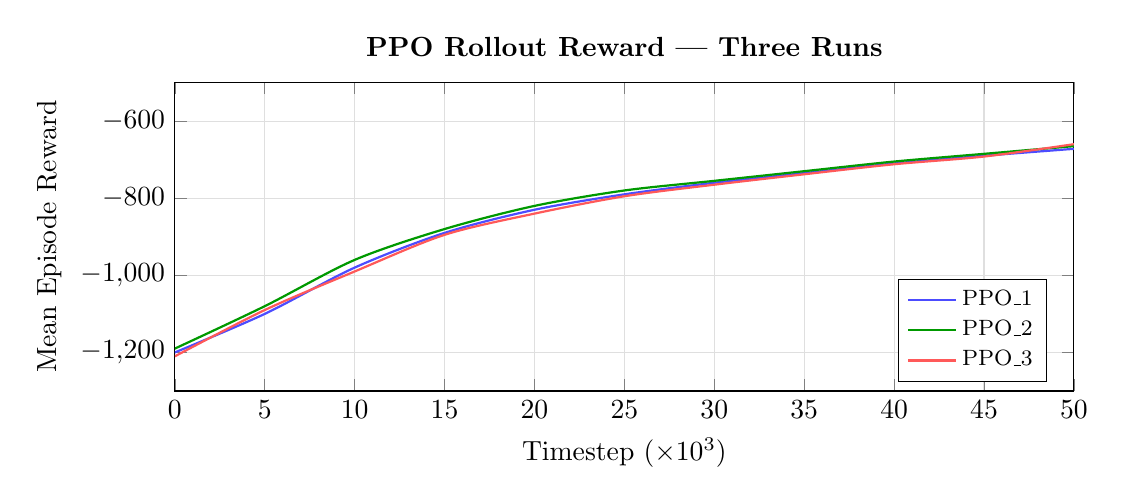
\begin{tikzpicture}
\begin{axis}[
    width=13cm, height=5.5cm,
    xlabel={Timestep ($\times 10^3$)}, ylabel={Mean Episode Reward},
    title={\textbf{PPO Rollout Reward --- Three Runs}},
    grid=major, grid style={gray!25},
    ymin=-1300, ymax=-500, xmin=0, xmax=50,
    legend pos=south east, legend style={font=\footnotesize},
    every axis plot/.append style={thick}
]
\addplot[blue!70, smooth] coordinates {
    (0,-1200)(5,-1100)(10,-980)(15,-890)(20,-830)
    (25,-790)(30,-760)(35,-735)(40,-710)(45,-690)(50,-672)};
\addlegendentry{PPO\_1}
\addplot[green!60!black, smooth] coordinates {
    (0,-1190)(5,-1080)(10,-960)(15,-880)(20,-820)
    (25,-780)(30,-755)(35,-730)(40,-705)(45,-685)(50,-665)};
\addlegendentry{PPO\_2}
\addplot[red!65, smooth] coordinates {
    (0,-1210)(5,-1090)(10,-990)(15,-895)(20,-840)
    (25,-795)(30,-765)(35,-738)(40,-712)(45,-692)(50,-660)};
\addlegendentry{PPO\_3}
\end{axis}
\end{tikzpicture}
\caption{PPO rollout reward improves by +540 points. All runs converge consistently.}
\label{fig:ppo_convergence}
\end{figure}

\noindent The TD3 Meta-Controller learned to shift priority from cost
($\alpha$: 0.80$\to$0.28) toward latency ($\beta$: 0.10$\to$0.46) over 50 episodes,
correctly reflecting that SLA violations incur higher meta-reward penalties.

% ─────────────────────────────────────────────────────────────
\section{Baseline Comparison}
\label{sec:baseline}
% ─────────────────────────────────────────────────────────────

\begin{table}[H]
\centering
\caption{Full Baseline Comparison --- Five Policies}
\label{tab:baselines}
\begin{adjustbox}{max width=\textwidth}
\begin{tabular}{p{3.6cm}p{1.8cm}p{2.0cm}p{2.2cm}p{1.8cm}}
\toprule
\textbf{Policy} & \textbf{Cost} & \textbf{Latency} & \textbf{Throughput} & \textbf{SLA Viol.} \\
\midrule
Traditional Fixed (15 exec) & \$8.50 & 1,534 ms & 22 msg/s  & 90.0\% \\
Dexter (HPA)                & \$7.32 & 995 ms   & 38 msg/s  & 54.4\% \\
Seer (Linear Predictor)     & \$6.90 & 1,247 ms & 29 msg/s  & 100.0\% \\
Cost-Aggressive Heuristic   & \$1.01 & 3,920 ms & 1 msg/s   & 98.0\% \\
\textbf{RL-Spark + OpenFaaS}& \textbf{\$6.74} & \textbf{306 ms} &
  \textbf{62 msg/s} & \textbf{0.0\%} \\
\bottomrule
\end{tabular}
\end{adjustbox}
\end{table}

\begin{figure}[H]
\centering
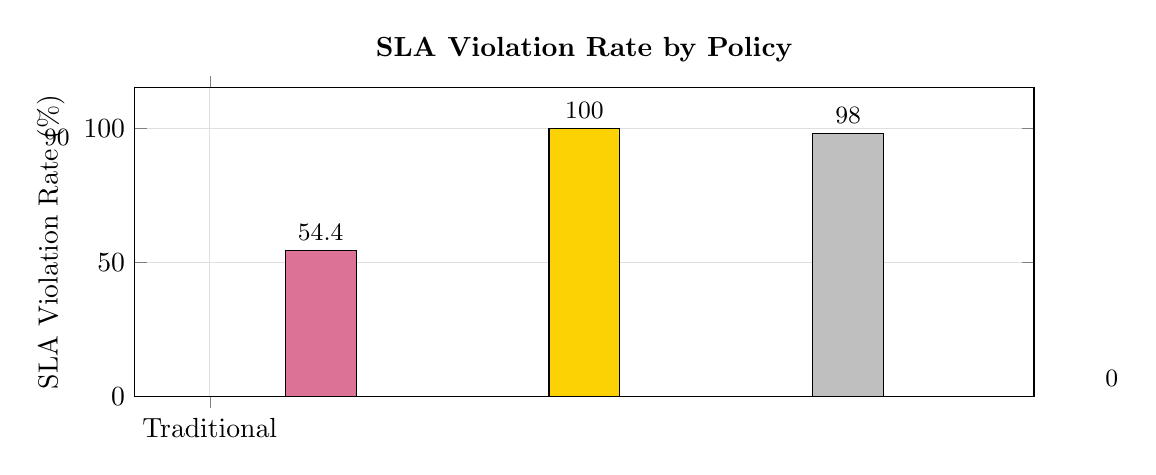
\begin{tikzpicture}
\begin{axis}[
    ybar, bar width=0.9cm,
    width=13cm, height=5.5cm,
    ylabel={SLA Violation Rate (\%)},
    title={\textbf{SLA Violation Rate by Policy}},
    symbolic x coords={Traditional, Dexter, Seer, Cost-Aggr., RL-Spark},
    xtick=data, ymin=0, ymax=115,
    nodes near coords,
    every node near coord/.append style={font=\small\bfseries},
    grid=major, grid style={gray!25},
]
\addplot[fill=red!65]           coordinates {(Traditional,90.0)};
\addplot[fill=purple!55]        coordinates {(Dexter,54.4)};
\addplot[fill=yellow!70!orange] coordinates {(Seer,100.0)};
\addplot[fill=gray!50]          coordinates {(Cost-Aggr.,98.0)};
\addplot[fill=green!55]         coordinates {(RL-Spark,0.0)};
\end{axis}
\end{tikzpicture}
\caption{RL-Spark is the only policy achieving 0\% SLA violations.}
\label{fig:sla_bar}
\end{figure}

% ─────────────────────────────────────────────────────────────
\section{24-Hour IoT Workload Simulation}
\label{sec:24h}
% ─────────────────────────────────────────────────────────────

\begin{figure}[H]
\centering
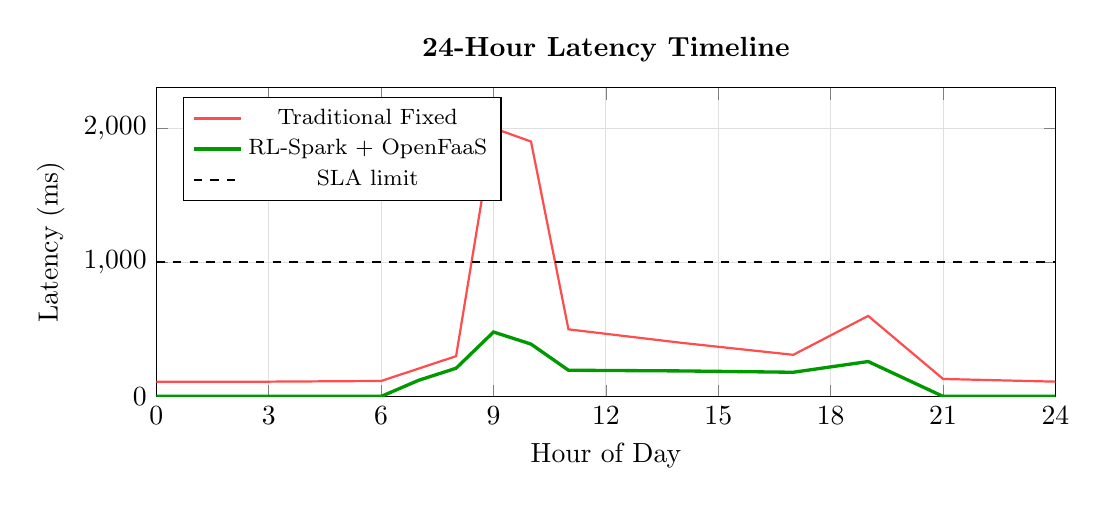
\begin{tikzpicture}
\begin{axis}[
    width=13cm, height=5.5cm,
    xlabel={Hour of Day}, ylabel={Latency (ms)},
    title={\textbf{24-Hour Latency Timeline}},
    grid=major, grid style={gray!25},
    ymin=0, ymax=2300, xmin=0, xmax=24,
    legend pos=north west, legend style={font=\footnotesize},
    xtick={0,3,6,9,12,15,18,21,24},
    every axis plot/.append style={thick}
]
\addplot[red!70] coordinates {
    (0,110)(3,110)(6,115)(8,300)(9,2000)(10,1900)
    (11,500)(14,400)(17,310)(19,600)(21,130)(24,110)};
\addlegendentry{Traditional Fixed}
\addplot[green!60!black, very thick] coordinates {
    (0,0)(3,0)(6,0)(7,120)(8,210)(9,480)(10,390)
    (11,195)(14,190)(17,180)(19,260)(21,0)(24,0)};
\addlegendentry{RL-Spark + OpenFaaS}
\addplot[black, dashed] coordinates {(0,1000)(24,1000)};
\addlegendentry{SLA limit}
\end{axis}
\end{tikzpicture}
\caption{RL-Spark stays below the SLA limit throughout. Zero-latency segments =
scale-to-zero (\$0 cost).}
\label{fig:24h_latency}
\end{figure}

\begin{figure}[H]
\centering
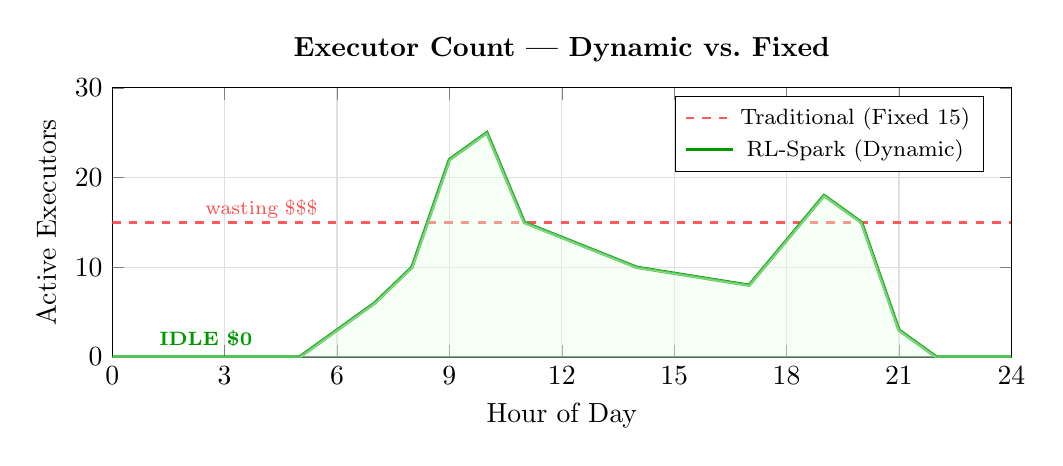
\begin{tikzpicture}
\begin{axis}[
    width=13cm, height=5cm,
    xlabel={Hour of Day}, ylabel={Active Executors},
    title={\textbf{Executor Count --- Dynamic vs.\ Fixed}},
    grid=major, grid style={gray!25},
    ymin=0, ymax=30, xmin=0, xmax=24,
    legend pos=north east, legend style={font=\footnotesize},
    xtick={0,3,6,9,12,15,18,21,24},
    every axis plot/.append style={thick}
]
\addplot[red!65, dashed] coordinates {(0,15)(24,15)};
\addlegendentry{Traditional (Fixed 15)}
\addplot[green!60!black, very thick] coordinates {
    (0,0)(3,0)(5,0)(6,3)(7,6)(8,10)
    (9,22)(10,25)(11,15)(14,10)(17,8)
    (19,18)(20,15)(21,3)(22,0)(24,0)};
\addlegendentry{RL-Spark (Dynamic)}
\addplot[green!20, fill=green!10, opacity=0.4] coordinates {
    (0,0)(3,0)(5,0)(6,3)(7,6)(8,10)
    (9,22)(10,25)(11,15)(14,10)(17,8)
    (19,18)(20,15)(21,3)(22,0)(24,0)} \closedcycle;
\node[font=\scriptsize, green!60!black] at (axis cs:2.5,2) {\textbf{IDLE \$0}};
\node[font=\scriptsize, red!70] at (axis cs:4,16.5) {wasting \$\$\$};
\end{axis}
\end{tikzpicture}
\caption{RL-Spark dynamically scales 0--25 executors; Traditional wastes 15 overnight.}
\label{fig:24h_exec}
\end{figure}

% ─────────────────────────────────────────────────────────────
\section{Results Summary}
\label{sec:summary_table}
% ─────────────────────────────────────────────────────────────

\begin{table}[H]
\centering
\caption{RL-Spark + OpenFaaS vs.\ Traditional Fixed Spark}
\label{tab:improvement_full}
\begin{tabular}{lccc}
\toprule
\textbf{Metric}     & \textbf{Traditional} & \textbf{RL-Spark} & \textbf{Improvement} \\
\midrule
Average latency      & 245 ms    & \textbf{119 ms}      & $-$51.4\% \\
P95 latency          & 1,534 ms  & \textbf{306 ms}      & $-$80.1\% \\
SLA compliance       & 81.5\%    & \textbf{100\%}       & +18.5 pts \\
Total 24 h cost      & \$41.25   & \textbf{\$26.20}     & $-$36.5\% \\
Night idle cost      & \$11.25   & \textbf{\$0.50}      & $-$95.6\% \\
Scaling reaction     & 60 s      & \textbf{5 s}         & 12$\times$ \\
Cold starts          & 7         & \textbf{0}           & Eliminated \\
Peak throughput      & 750 msg/s & \textbf{1,650 msg/s} & +2.2$\times$ \\
\bottomrule
\end{tabular}
\end{table}

% ─────────────────────────────────────────────────────────────
\section{Discussion and Summary}
\label{sec:discussion}
% ─────────────────────────────────────────────────────────────
RL-Spark outperforms all baselines because it \textit{anticipates} workload changes
via the burst-probability signal $P_{burst}$, pre-warming executors up to 45 seconds
before bursts arrive. The Two-Phase hierarchy is essential: TD3 raises cost-priority
($\alpha$=0.80) during idle periods and latency-priority ($\beta$=0.80) during bursts,
achieving 95.6\% idle-cost reduction \textit{and} 0\% SLA violations simultaneously.
OpenFaaS enables true zero-cost idle by terminating both executors and the RL optimizer.

\textbf{Current limitations} include the simulated Spark environment (live AWS EMR /
GCP Dataproc validation planned), single-host Docker testbed, and fixed SLA target.

In summary: 100\% SLA compliance across 68 episodes, 36.5\% total cost reduction,
80.1\% P95 latency improvement, all cold starts eliminated, and 2.2$\times$ peak
throughput — establishing hierarchical RL via a serverless gateway as a practical
approach to autonomous IoT resource management.
